% Chapter Template

\chapter{Introduction} % Main chapter title

\noindent\textbf{\large Contents:}

\noindent\hrulefill
\noindent\startcontents[chapters]
\noindent\printcontents[chapters]{}{1}{}
\noindent\hrulefill

\label{Chapter1} % Change X to a consecutive number; for referencing this chapter elsewhere, use \ref{ChapterX}




The advancement of Astronomy has always been closely linked to achieving higher
resolution.  Early on, this was a conceptually easier concept.  The bigger your
telescope aperture, the more light can be collected.  With early telescopes this was
limited by how large of lens a manufacturer could make.  Eventually lenses became so
large that they can collapse under their own weight.  Next, a way to make mirrors
that did not tarnish too quickly became available.  Mirrors could be supported from
the back, allowing for large mirrors.  When single mirror systems became too heavy,
segmented mirror designs were created in order to have an almost limitless aperture
size.  

\begin{figure}[h!]
\centering
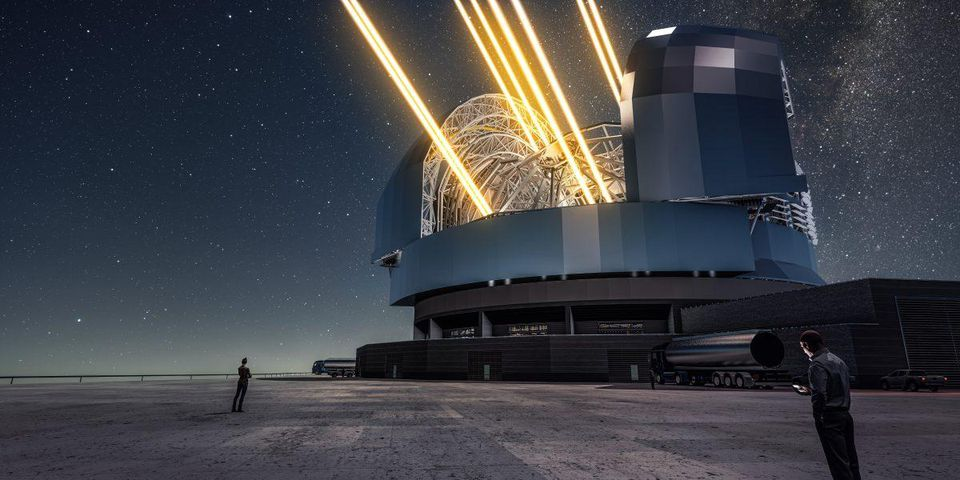
\includegraphics[width=14cm]{Figures/ELT_las.jpg}
\caption{Artist representation of the ELT}
\label{fig:ELT_las}
\end{figure}

%Expand on atmosphere interfereing with light
% Talk about why large apertures need AO
% Talk about Strehl ratio

However, the Earth's atmosphere interferes with light, widening the PSF of an  
object.  This is also known as seeing limited observations.  Now with the new
generation of 25+ meter telescopes, a way to make diffraction limited observations
is more necessary than ever.  Wavefront errors can be calculated using the "Fried
Parameter" or $r_0$.  $r_0$ is defined as the largest distance on a telescope primary
over which the phase of an incoming wave is well-correlated \cite{max_2019}.  The Fried
Parameter at good cites is roughly equal to 10 to 15 microns \cite{max_2019}.  As telescope diameters become larger 

\begin{figure}[h!]
\centering
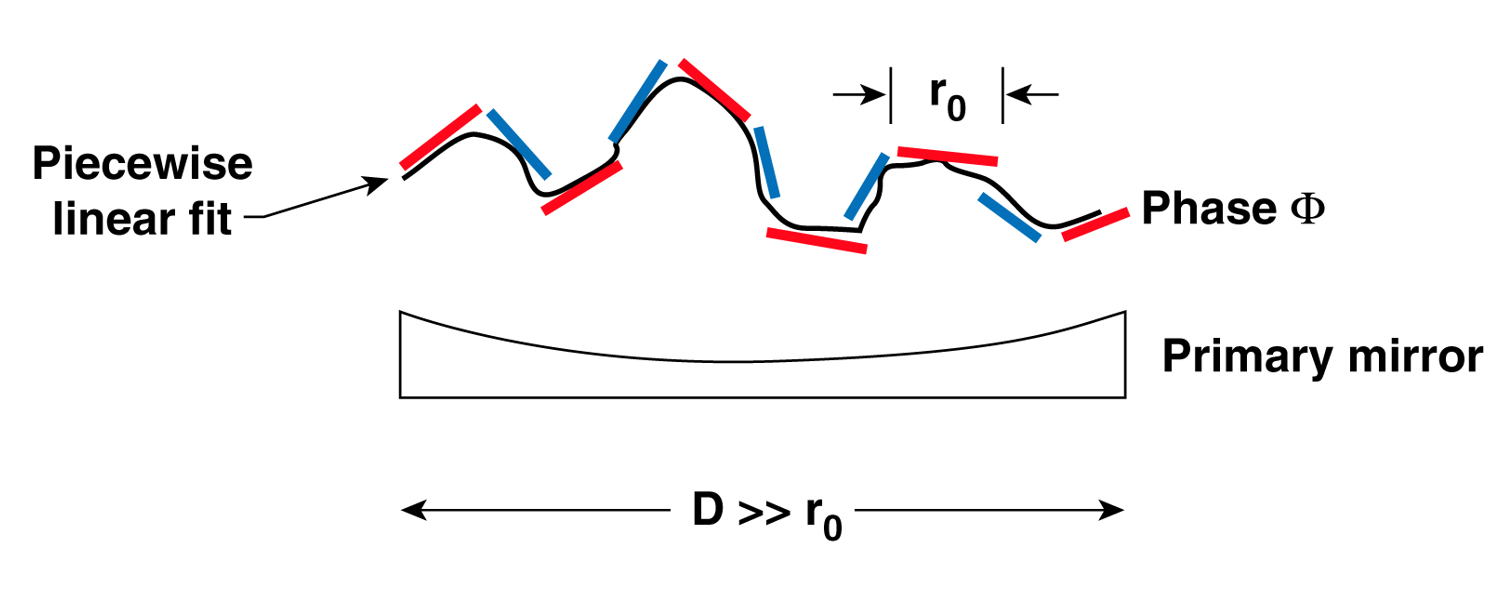
\includegraphics[width=14cm]{Figures/r0.png}
\caption{Example of a distorted wavefront and where the Fried Parameter ($r_0$) can fit on the wavefront.}
\label{fig:ELT_las}
\end{figure}

Adaptive optics is the use of matching the wavefront errors  
with deformable mirrors to increase the Strehl Ratio of a given observation.  The  
Mid-Infrared ELT Imager and Spectrograph or METIS, looking to take advantage of the
ELT's 39 meter aperture to explore the mid-infrared sky.  In order to do so, METIS
must perform wavefront sensing to control the adaptive secondary.


\section{History of Adaptive Optics}


Light observed from astronomical sources travels anywhere from light years to
billions of light years to our ground based detectors.  Usually travelling mostly
unimpeded through out that entire journey.  It isn't until the last 100 kilometers
that the light gets distorted by our atmosphere.  The change from vacuum to the
medium that is our atmosphere causes the light to refract.  However, the atmosphere
is not homogeneous.  The atmosphere has temperature fluctuations and mixing currents
that cause difference in indices of refraction and path length of incoming light.

%Is throughout one word?

Now that telescopes can be made to be eight meters and bigger,
being able to correct for the Earth's atmosphere is necessary 
to advance ground based astronomy.  First attempts to get around the atmosphere's 
interference with incoming light was the speckle imaging technique.  The idea was 
to take short exposures of the target in order to limit the effects of the
atmosphere.

This technique allowed for countless discovery of binary star systems that were
otherwise observed as singular stars.  This lead to the discovery of multiple binary
star systems that were otherwise assumed to be one star.  This produced images, like
the one above.  However, this technique could only be used on bright objects that
could be exposed in under 100ms.  (Should do a little more research here).  This
means that there is still a large part of the night sky that we cannot observe using
this technique.

\begin{figure}[h!]
\centering
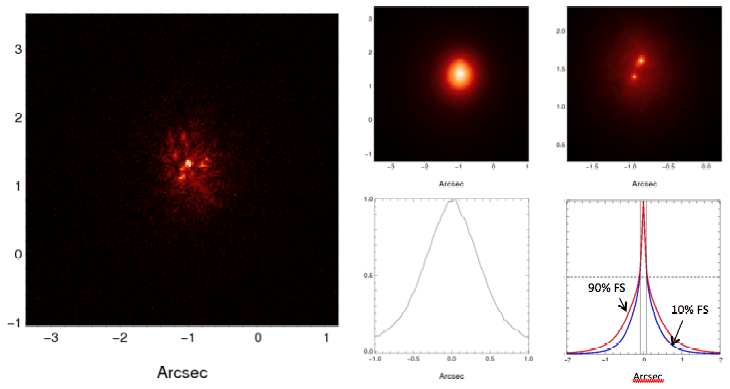
\includegraphics[width=14cm]{composite3.png}
\caption{Here we can see using the Speckle technique that there are actually two stars in what was previously believed to be one star.}
\label{fig:speckle}
\end{figure}


In order to advance imaging techniques, it became necessary to reconstruct the
wavefront as it was before it encountered the atmosphere. Because the atmosphere distorts the
wavefront, it should be feasible to match the wavefront to correct for the
aberrations to the wavefront.  This is done by having a deformable, reflective
membrane.  These are called deformable mirrors (DM). DM's are responsible for
reconstructing the wavefront errors in the atmosphere to counter the phase
differences, thus reconstructing the image (Figure \ref{fig:AO_no_AO}).

\begin{figure}[h!]
\centering
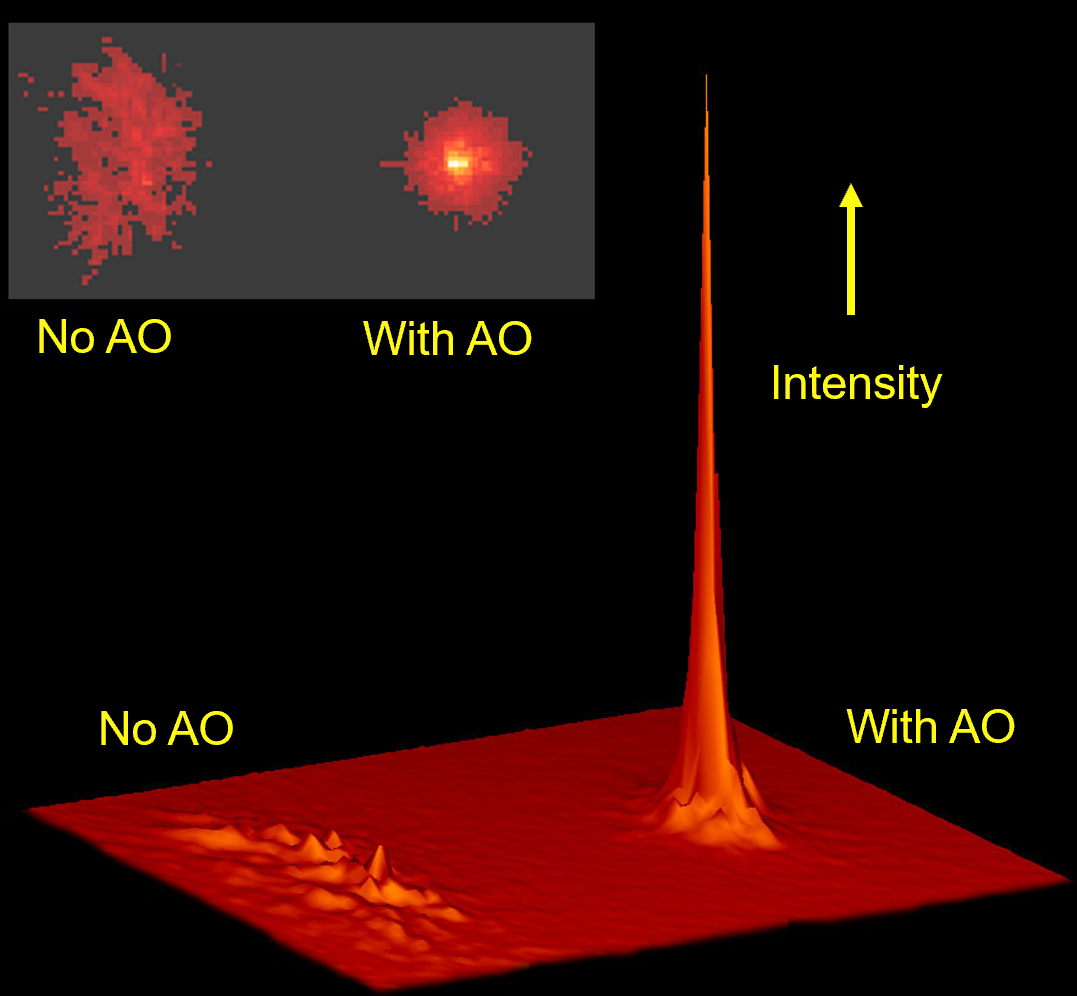
\includegraphics[width=10cm]{Figures/AO_vs_no_AO.png}
\caption{Here we can see the clear difference between the AO corrected image and no AO correction.}
\label{fig:AO_no_AO}
\end{figure}


In order for DMs to accurately match the wavefront error, there needs to be an
additional calibration source.  This can be done a few ways.  The ways covered in
this thesis will be Single Conjugate Adaptive Optics (SCAO), Single Laser Adaptive
Optics (SLAO), and Laser Tomography Adaptive Optics (LTAO).


\section{Single Conjugate Adaptive Optics}

Adaptive Optics, in order to work, needs a reference source to measure the
disturbances of the Earth's atmosphere.  In this case, we look at a Natural Guide
Star (NGS).  An NGS is a sufficiently luminous star that can be used for wavefront
detection.  In the case of METIS, it was determined that a magnitude 10 star in the
K-band would be needed for sufficient wavefront correction \cite{star_mag}.  The
sufficiently bright star properly illuminates the entrance pupil to be measured by a
wavefront sensor (WFS).  Currently there are two methods to measure wavefront error
(Figure \ref{fig:scao}).  

\begin{figure}[h!]
\centering
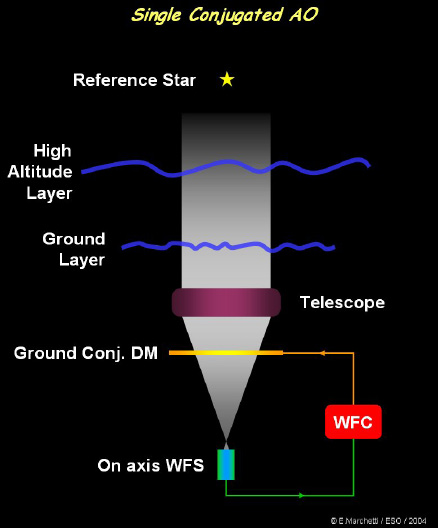
\includegraphics[width=8 cm]{scao.jpg}
\caption{Representation of Single Conjugate AO\cite{aomode}.}
\label{fig:scao}
\end{figure}

First is a Shack-Hartmann Wavefront sensor.  This method uses a lenslet array to
subdivide the pupil plane to measure deviations from a planar wavefront.  This is
done by measuring deviations from a grid of spots created by the lenslet array
(Figure \ref{fig:Micro_lens_array}).  This is the current method METIS will be doing
wavefront sensing and will be covered in Chapter \ref{Chapter3}.

\begin{figure}[h!]
\centering
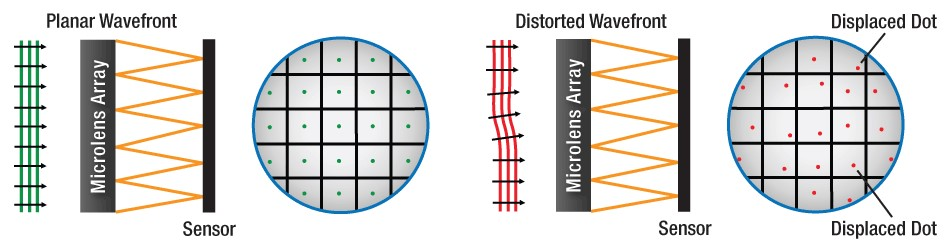
\includegraphics[width=14cm]{Figures/MLA.jpg}
\caption{An example of a lenslet array with wavefront error.}
\label{fig:Micro_lens_array}
\end{figure}

The second is a Pyramid Wavefront Sensor (PWS).  PWS works by focusing light to the
tip of a pyramid made of glass to subdivide the aperture into four segments.  The
detector is placed at the pupil plane and directly images the pupil (Figure
\ref{fig:pyramid}).  The advantage here is that the light is divided only 
four times.  This means that the NGS can be a higher magnitude and still allow for
AO corrections \cite{Shatokhina:13}.  METIS will not be using a PWS and will instead
use a SHWFS.

\begin{figure}[h!]
\centering
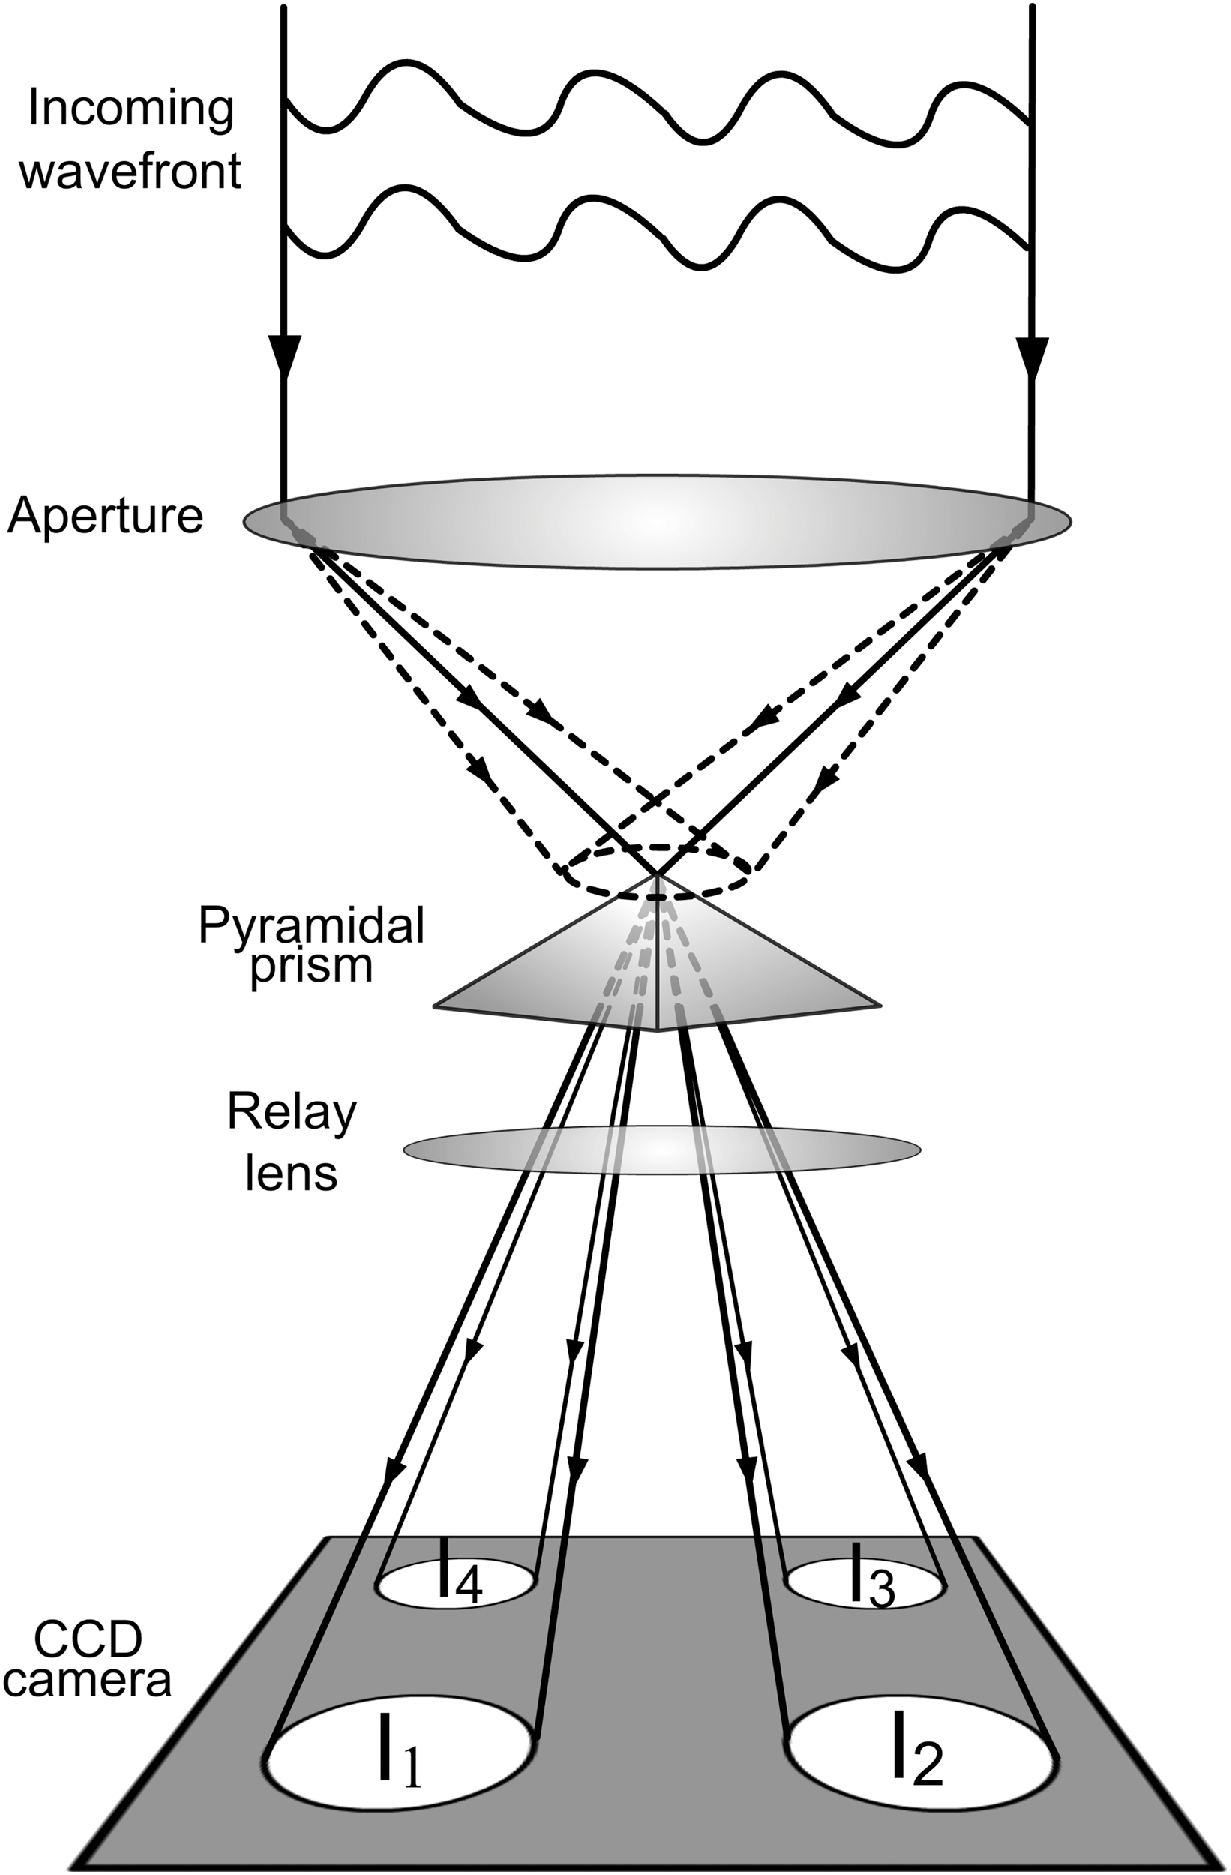
\includegraphics[width=8cm]{Figures/pyramid.jpeg}
\caption{An example of a pyramid wavefront sensor \cite{Shatokhina:13}.}
\label{fig:pyramid}
\end{figure}

% Talk more about PWF

One of the big advantages of Single conjugate AO is that star light comes from
outside the Earth's atmosphere.  This means that, to first order, wavefronts are
planar and that the same source can be used for tip/tilt measurements.  This will be
an issue when using Laser Guide Stars (LGS).  One thing effects SCAO systems is
anisoplanetism.  This is when a NGS is off-axis from the observed object.  This will
lead to residual wavefront error that is not in line with the observed object since
the two different sources go through different parts of the Earths atmosphere.  This
is illustrated in Figure \ref{fig:ani}.

However, the night sky is not filled with sufficiently bright stars.  Especially for
extra-galactic observations, there is a need for bright sources.  An
artificial star is necessary for these types of observations.  This is where laser
guide stars come in.

% Here's the image code:
\begin{figure}[h!]
\centering
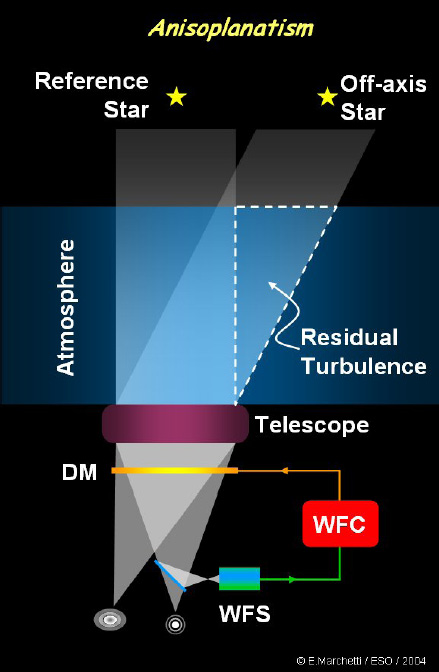
\includegraphics[width=6 cm]{anisoplanetism.jpg}
\caption{Here we can see an example of turbulence picked up by off axis-star but not the Reference star\cite{aomode}.}
\label{fig:ani}
\end{figure}




\section{Single Laser Adaptive Optics}

Single laser Adaptive Optics (SLAO) is the practice of using a Laser Guide Star
(LGS) in order to illuminate the night sky to have enough illumination on the
entrance pupil of the telescope.  Nowadays, the main type of laser used in astronomical
adaptive optics is the sodium laser.  The top of the Earth's atmosphere has a 10 km
thick layer of sodium approximately 90 km above sea level \cite{sodium}.  This is
the highest altitude an artificial star can be.  The other laser type, the Rayleigh,
laser has a height of roughly 20-40 km above sea-level \cite{Rayleigh}.  % Talk more about how this is possible

Sodium lasers excite sodium atoms in the upper atmosphere and emit at 589 nm.  The
advantage of having the laser higher in the atmosphere is that it limits the cone
effect.  The cone effect is where there is residual turbulence not picked up by the
laser spot (Figure \ref{fig:cone}).  This is not always a full proof method though.
The sodium layer is not a uniform and constant layer.  On a time scale of hours, the
thickness, height, and density of the sodium layer can change \cite{sodium}.  This
will lead to variations in intensity of the LGS.

Laser guide stars also are not capable of providing tip/tilt measurements.  This is
due to the fact that the laser both travels up and back down in the atmosphere.  
This means that an off-axis star is required to provide tip/tilt measurements. 
However, the star can be higher in magnitude since the star is not needed for
wavefront correction.

%Reference FIgs
\begin{figure}[h!]
\centering
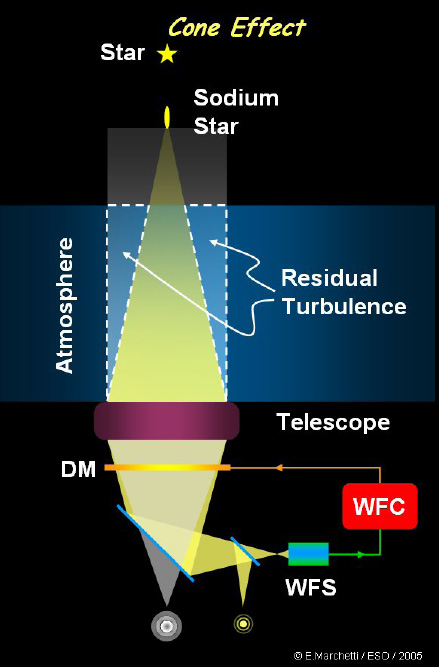
\includegraphics[width=6 cm]{cone_effect.jpg}
\caption{A figure of SLAO.  Note where the laser light does not cover.  This is the cone-effect, where there is residual turbulence not corrected\cite{aomode}.}
\label{fig:cone}
\end{figure}

While taking an AO class with Claire Max at UC Santa Cruz, she described SLAO is
"like looking through a straw".  The correction done by SLAO provides correction but
for a small FoV.  This is in part due to the cone effect of SLAO observations.  New
techniques have come about to limit the cone effect and expand the FoV for laser AO
systems.  Some examples are Ground Layer AO (GLAO), Multi-conjugate AO (MCAO),
Multi-Object AO (MOAO), and Laser Tomography AO (LTAO).  METIS was originally
designed for LTAO corrections.


\section{Laser Tomography Adaptive Optics}

Laser Tomography is the practice of using multiple laser guide stars to illuminate
different layers of the atmosphere in order to reconstruct aberrations at each
layer.  This means there is one WFS per LGS since each LGS is conjugate to a
different layer.  LTAO does provide better performance with wavefront reconstruction
as well as widening the FoV of observations.  An illustration of LTAO can be seen in
Figure \ref{fig:tomo}.

LTAO does however take a lot more time, money, and space to implement.  All of which
are critical aspects of any project.  ELT has 6 laser guide stars, which would mean
6 wavefront sensors.

\begin{figure}[h!]
\centering
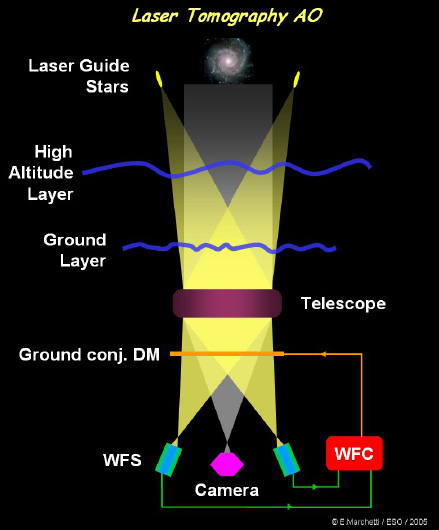
\includegraphics[width=8 cm]{laser_tomo.jpg}
\caption{A Figure of a laser tomography set up.  Here two lasers measure two different layers and measured by two different WFS to correct a Ground conj. DM. \cite{aomode}}
\label{fig:tomo}
\end{figure}

\section{METIS Science Goals}

The Mid-infrared ELT Imager and Spectrograph (METIS) goal is to explore the L-
(2.9-4$\mu$m), M-(4.6-5$\mu$m), and N-(7.5-13$\mu$m) bands using the Extremely Large
Telescopes (ELT) 39 meter aperture.  The main goal for METIS is to explore
proto-planetary regions.  This allows for the central star to be used as the main
source for wavefront detection.  A layout of MEITS can be seen in Figure
\ref{fig:metis_over}.  However, METIS can be used to explore many regions
of the night sky outside of exo-planet discovery.  Because METIS will be one of the
few instruments with mid-IR seeing, it would be of great benefit to have METIS
observe extra-galactic objects.  These observations would more than likely require
the use of a laser guide star (LGS) in order to do wavefront sensing.  Originally it
was thought that METIS would use the full suite of lasers that comes with the ELT,
however due to constraints in budget, size and weight, it was considered looking
into whether or not using a single laser would be just as effective.

\begin{figure}[h!]
\centering
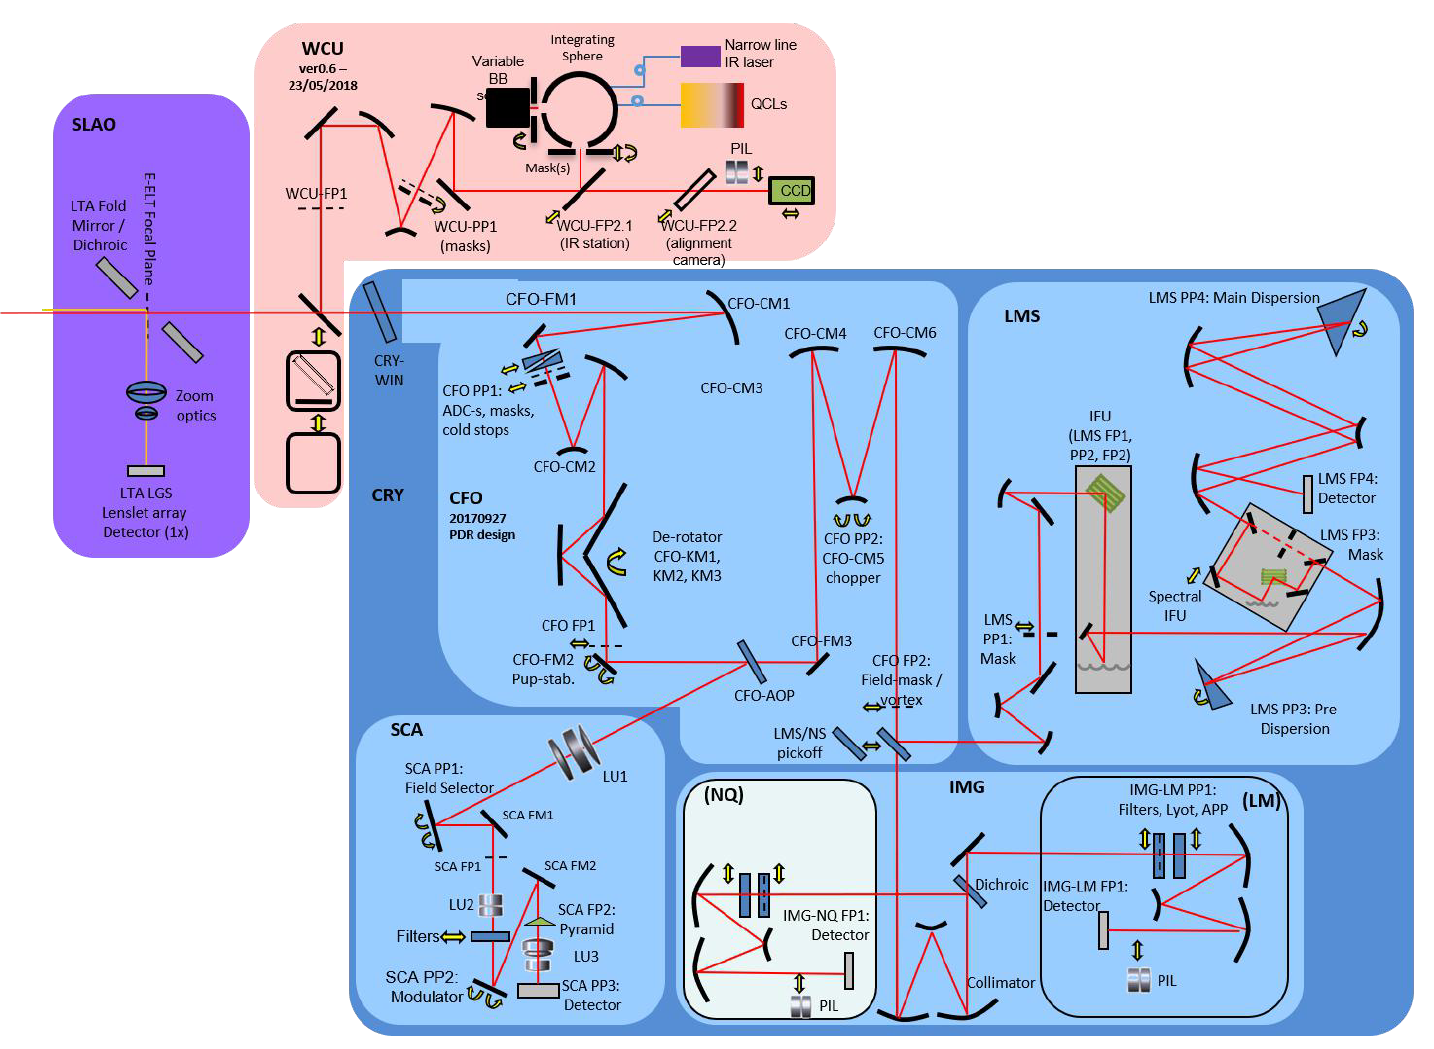
\includegraphics[width=12 cm]{Figures/METIS_SLAO.png}
\caption{A systematic representation of METIS including its proposed SLAO system \cite{METISSPIE2016}}
\label{fig:metis_over}
\end{figure}

The advantages of using a single laser are that the cost would be dramatically
reduced only sensing one layer rather than having multiple wavefront sensors. 
Having multiple wavefront sensors means more optics, which entails more space and
more cost.  The size limitations to the wavefront sensor are from the position of
METIS from the pre-focal station of the ELT nasmyth platform.

Because METIS is a infrared instrument, we need to pick off the incoming laser light
with the use of as little optics as possible.  Using a beam-splitter dichroic is one
option.  The idea would be that the dichroic would allow the infrared light to pass
through while sending off the light from the laser off to the wavefront sensor. 
However, since the AO system will be outside of the chryostat, the optic will be
relatively warm.  This would add to the noise of the instrument.  Instead, we use
the fact that the laser and the science objects will have different foci.  The
solution of an annular mirror was brought up.  This would act as a beam-splitter,
allowing the science light to pass through a central hole in a mirror while picking
up off the light from the laser, sending it off to the wavefront sensor.

\section{Focus of the Thesis}

The new class of extremely large telescopes (25+ meter) needs to use adaptive optics
in order to take advantage of the full aperture size.  Originally, METIS was posed
to use LTAO.  However, since cost is always a large factor in any project, it was
worth looking into using a SLAO system.  This work was done by a previous student,
Benjamin Arcier.  His work showed acceptable performance by a SLAO system for METIS.
From this, an initial optical design was made and can be seen in Figure
\ref{fig:ben_optic}.  However, it was shown to be costly.  The design had all
aspherical surfaces from large optics to very small.  All of which are possible to
make, however they are quite expensive due to the manufacturing process in
which aspherical components are made.  Spherical surfaces however are much cheaper
to manufacture.



\begin{figure}[h!]
\centering
\begin{subfigure}{.5\textwidth}
  \centering
  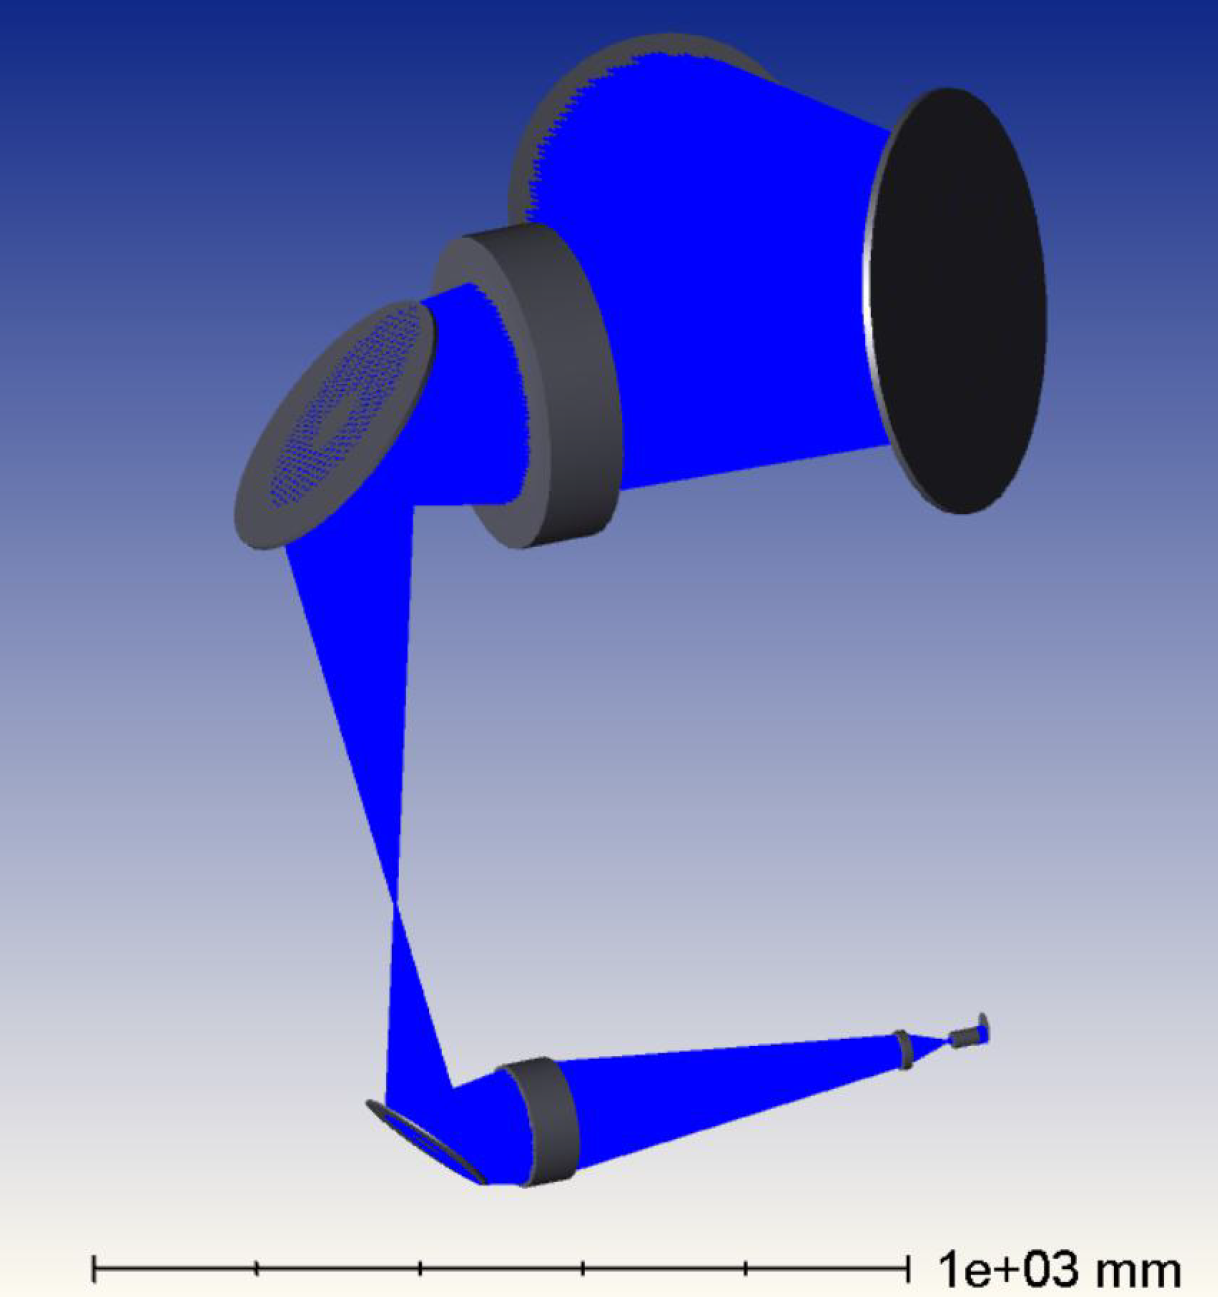
\includegraphics[width=6cm]{Figures/Ben_optic_design.png}
  \caption{A shaded model of Benjamin Arcier's optical design.  Light comes from the top right and folds down to a camera on the bottom right}
  \label{fig:ben_optic}
\end{subfigure}%
\begin{subfigure}{.5\textwidth}
  \centering
  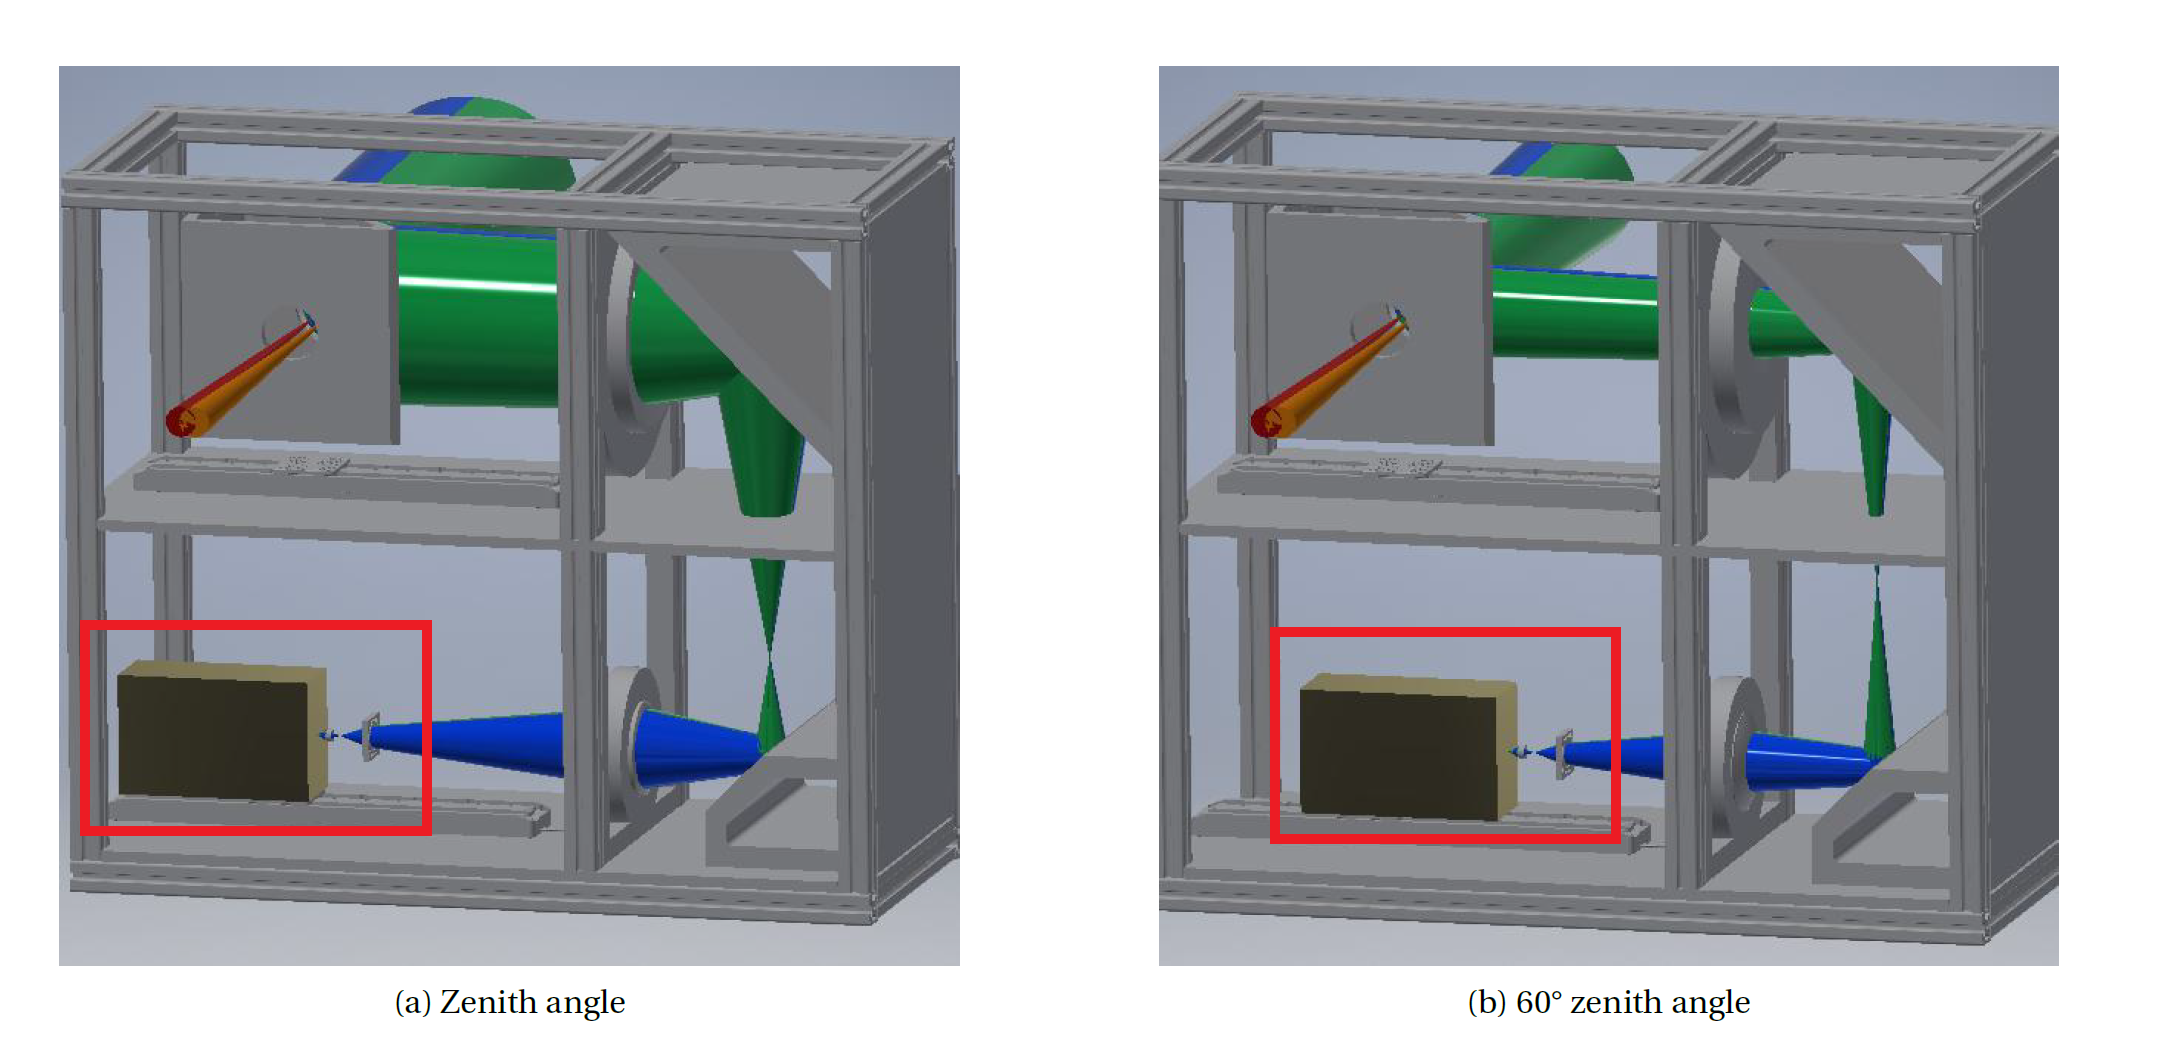
\includegraphics[width=8cm]{Figures/camera_change.png}
  \caption{A figure showing how the original design compensated for the change in focus.  All objects in the red square were on a moving stage}
  \label{fig:camera_change}
\end{subfigure}
\caption{Figure showing the end result of Benjamin Arcier's research.\cite{arcier}}
\label{fig:pickup}
\end{figure}

Another issue was the way the system dealt with the change in focus from telescope
elevation angle change.  The design had the camera and two separate optics mounted
to a moving platform to compensate for the changing distance of the laser spot. 
This presents a problem.  With the camera attached to the moving stage, so does the
additional cabling.  This could wear down the cables insulation and could lead to
failures.  Because of this, it is important to implement a simple way to compensate
for the change in laser distance with as few moving parts as possible.

The focus of this thesis is to explore these issues by looking at different optical
concepts to produce a more manufactureable design.  This included looking into
mirrored systems for magnification and adding more optical surfaces to manipulate
the light path.  There should also be a simple mechanism to adjust for the change in
focus of the laser spot with as few moving optical surfaces as possible.  After the
optical design is complete, the next step was to construct a first order
opto-mechanical design to fit within the space envelope between METIS and the
prefocal station of the ELT.




%----------------------------------------------------------------------------------------
%	SECTION 1
%----------------------------------------------------------------------------------------
